\section{Generalità delle fratture}

\subsection{Introduzione}
La pratica ortopedica risale a epoche lontane eppure la parola "ortopedia" viene usata solo dal 1741: fu coniata dal medico francese Nicolas Andry, a partire da due parole greche (orthòs: diritto; pàis: bambino) perché aveva come obiettivo quello di correggere le deformità del fisico nei bambini.
Questa disciplina si è sviluppata soprattutto durante le guerre che fornirono molti casi traumatologici su cui "sperimentare".
Altri eventi che hanno contribuito allo sviluppo di tale disciplina sono stati l'avvento delle moderne tecniche anestesiologiche, della radiologia e degli antibiotici.
Oggi la traumatologia e l'ortopedia sono sostenute in maniera significativa dalla tecnologia. Per rendersi conto dell'importante contributo di quest'ultima alla pratica ortopedica basti ricordare che i materiali prima usati su aerei militari e aerei civili, sono ora parte delle protesi usate in ortopedia.
Grandi speranze sono riposte nella biotecnologia, nelle ricerca sulle cellule staminali e sui fattori di crescita che in parte sono già utilizzati, ma di cui ci si augura di poter sfruttare al massimo le potenzialità nel futuro. Noi (futuri) medici abbiamo il dovere di
informarci su questi nuovi orizzonti per dare al paziente consigli giusti e per offrire la migliore soluzione sul piano terapeutico.

\subsection{Definizione e trattamento}
Una frattura è definita come una \emph{soluzione di continuità di un segmento osseo} conseguente ad un trauma che agisce sul segmento stesso.
La forza e l'energia meccanica del trauma (perché si abbia tale frattura) devono essere di intensità tale da superare i limiti di deformabilità e resistenza del segmento osseo colpito così da determinarsi la frattura. (Ad esempio, un motociclista che cade e urta
contro un palo è quasi certo che avrà una frattura).

\begin{figure}[!ht]
\centering
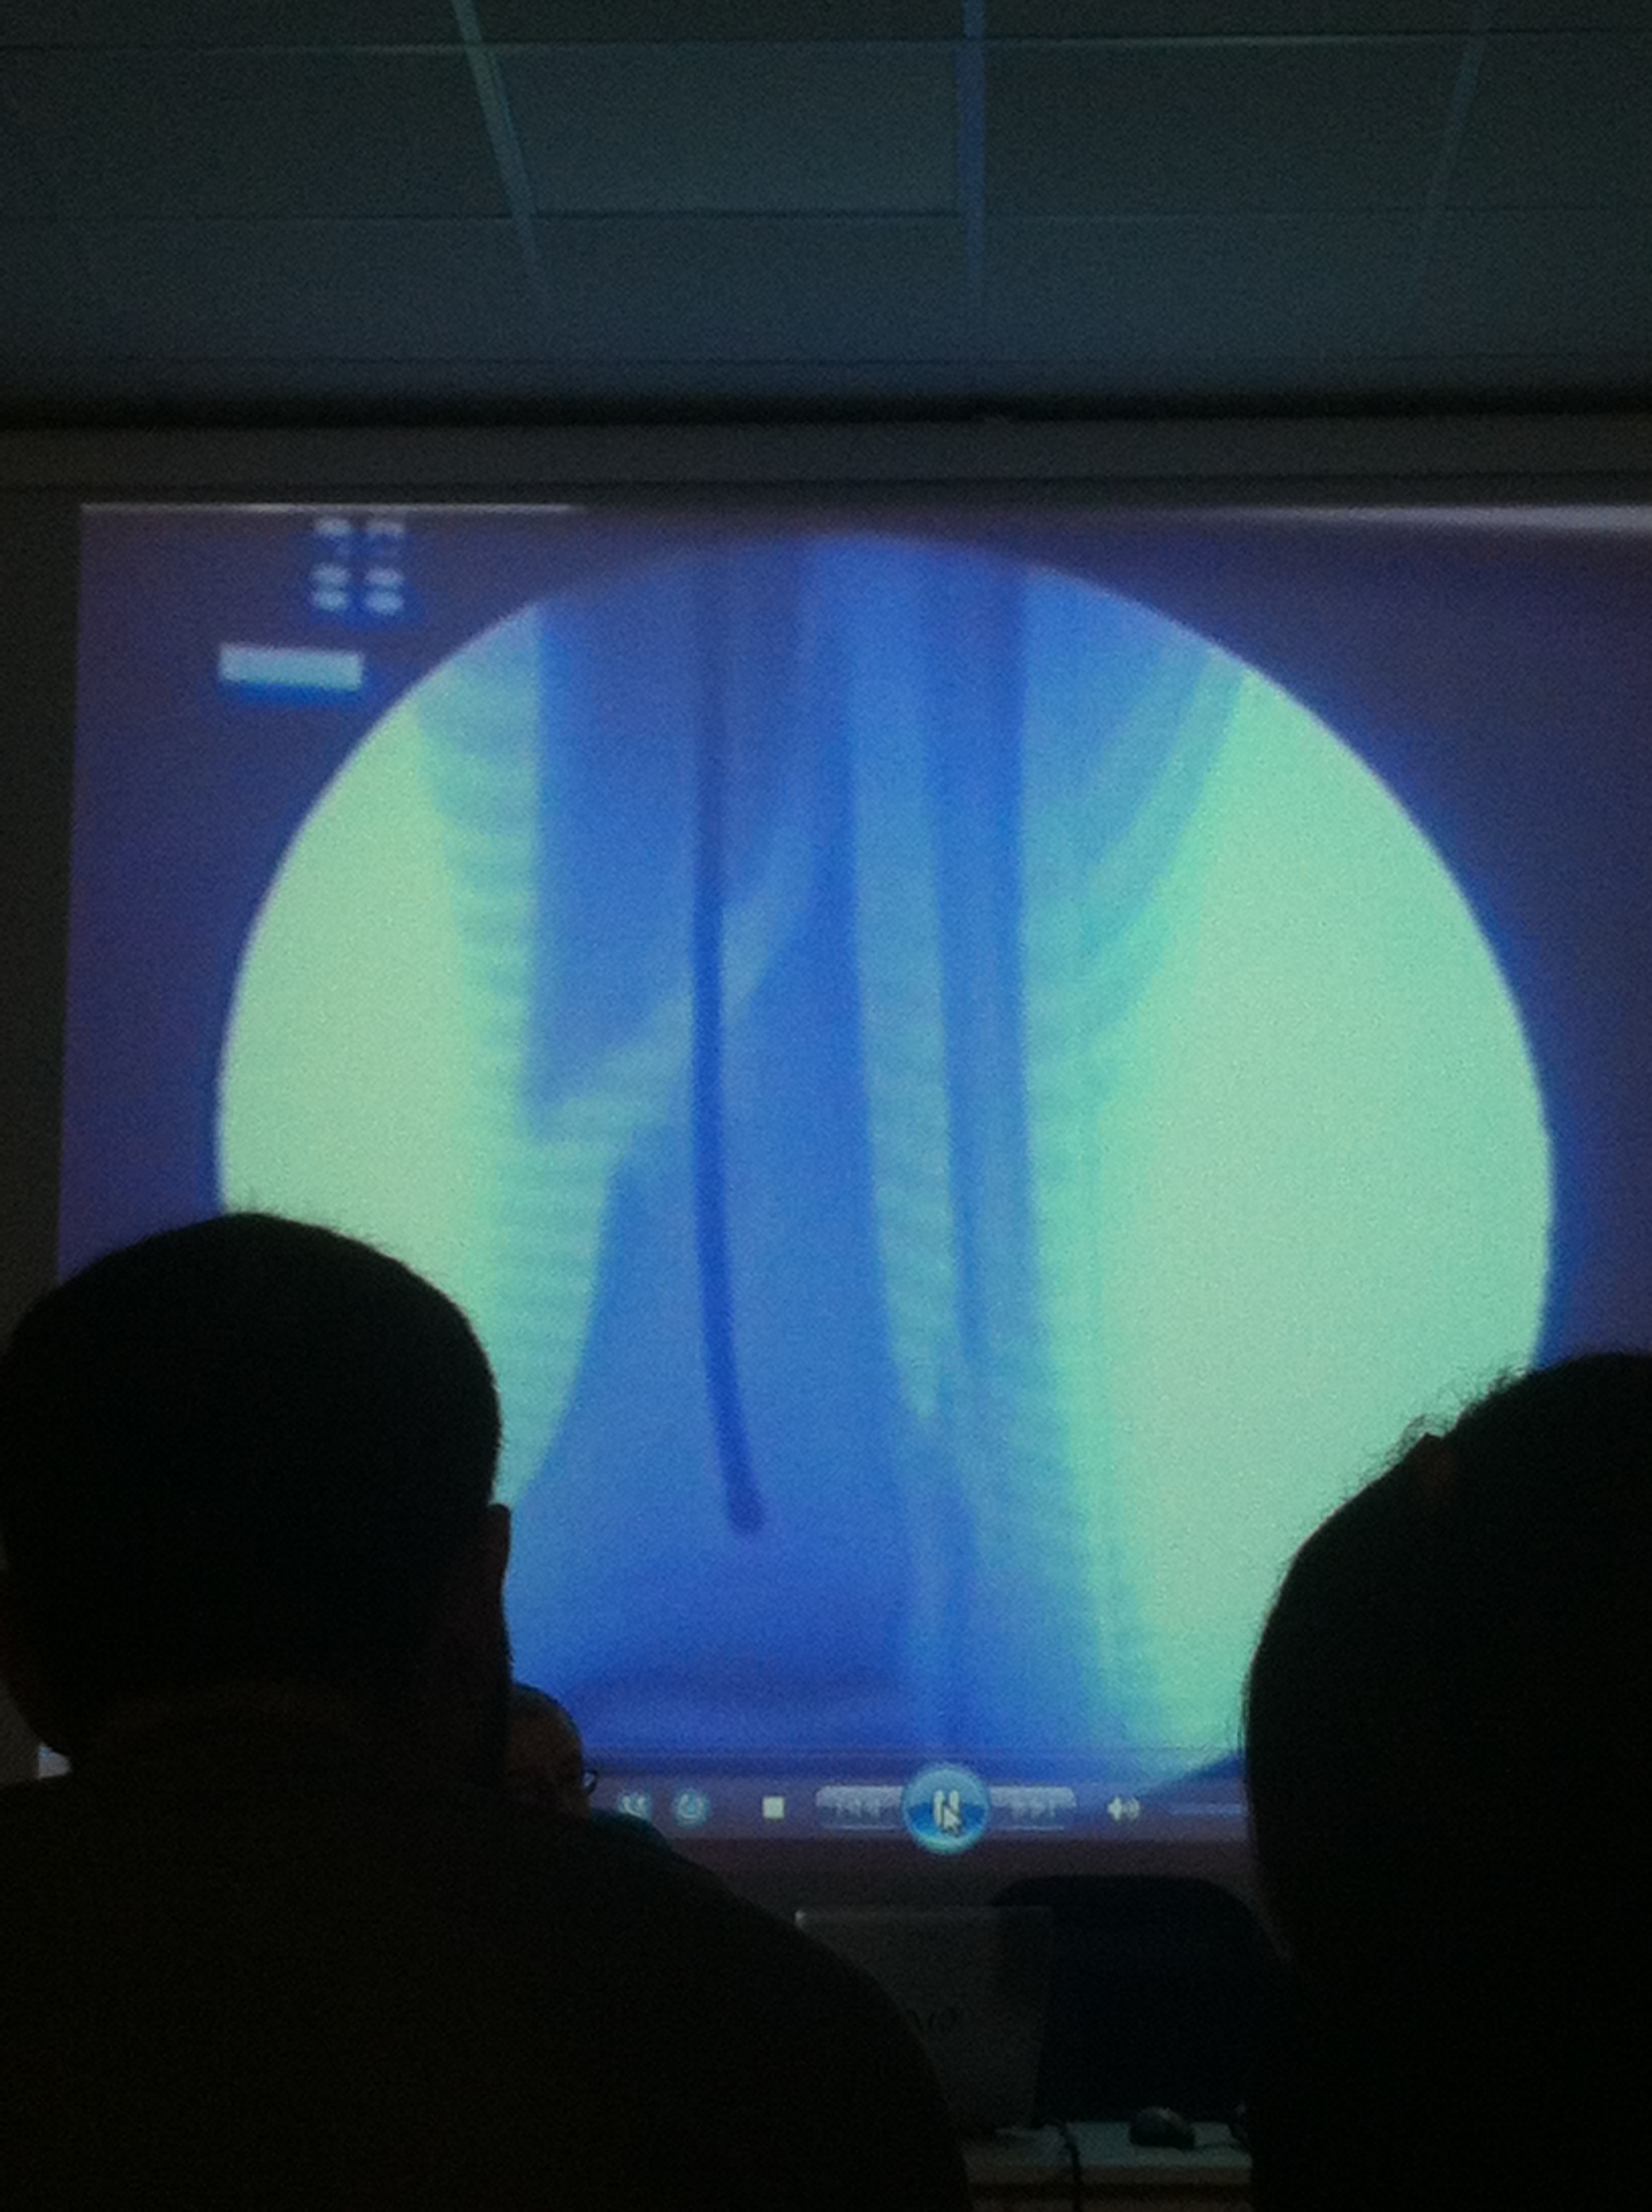
\includegraphics[width=0.3\textwidth]{001/image1.jpeg}
\end{figure}

Le fratture possono essere suddivise in:
\begin{itemize}
\item
  \emph{Traumatiche}
\item
  \emph{Patologiche, e ``da fragilità''}
\item
  \emph{Da stress (o da durata)}
\item
  \emph{Iatrogene (osteotomie)}
\end{itemize}



Nell'immagine: radiografia della gamba che mostra un segmento osseo discontinuo. Si tratta di una frattura del terzo distale della tibia e del terzo distale del perone.


\subsection{Diagnosi ( questa parte è stata ripresa e approfondita nella lezione del
08-03 )}

Per la diagnosi di frattura vanno sempre considerati più aspetti.

\subsubsection{Segni di probabilità}

\begin{itemize}
\item
  Atteggiamento: un paziente con un arto (o l'intero corpo) in posizione antalgica può far sospettare una frattura; ad esempio l'atteggiamento tipico delle fratture del collo del femore: l'arto è extra ruotato, addotto e accorciato
\item
Deformità grossolane, ad esempio la gamba in un senso e il piede nell'altro
\item
Lesioni cutanee e tumefazioni
\item
 Impotenza funzionale
\item
 Dolore
\end{itemize}

\subsubsection{Segni di certezza}

\begin{itemize}
\item
 Crepitio: la cauta mobilizzazione del segmento evoca il rumore delle superfici ossee a confronto
\item
 Motilità preternaturale
\end{itemize}

Per la \textbf{diagnosi definitiva} ci si avvale delle tecniche radiologiche: inizialmente radiografica, eventualmente TC o RM (se dovessero permanere dubbi o in caso si sospettino lesioni ai tessuti circostanti).

Nel momento in cui si ha un sospetto di frattura occorre procedere come di seguito:

\begin{itemize}
\item
  Immobilizzazione provvisoria sul luogo dell'incidente
\item
  Radiografia convenzionale (che permette la diagnosi di frattura).
N.B. La radiografia permette anche di definire e analizzare le caratteristiche di tale frattura
\item
  Trazione se necessario
\end{itemize}


\subsection{Trattamento}

Una volta fatta diagnosi di frattura inizia il processo di \textbf{riparazione della frattura}. \emph{Il trattamento delle frattura ha come scopo il recupero funzionale completo del segmento fratturato senza deformità residue o alterazioni significative della morfologia scheletrica e con il pieno recupero della funzione muscolare e articolare.}

Ci sono due aspetti da considerare e che garantiscono la guarigione di una frattura:

\begin{itemize}
\item
  \textbf{Riduzione della frattura}: si tratta del complesso di manovre messe in atto nel caso di frattura scomposta o fratture-lussazioni al fine di riposizionare i segmenti ossei nella corretta posizione anatomica. Tale manovra viene può essere eseguita dall'ortopedico manualmente ed è appunto detta manuale oppure essere eseguita chirurgicamente. A seguito di questo bisogna procedere con la stabilizzazione.

\item
  \textbf{Stabilizzazione} dei vari elementi della frattura. Si attua per mezzo di un apparecchio gessato o chirurgicamente attraverso l'utilizzo di diversi mezzi di sintesi in genere mezzi metallici tramite cui si fissa la frattura una volta che è stata ridotta. Tali mezzi di sintesi comprendono viti metalliche, placche associate a viti, chiodi endomidollari, fissatori esterni, fili metallici che passano attraverso la cute e bloccano la frattura.
\end{itemize}

In base alle modalità per cui si opta distinguiamo un \textbf{\emph{trattamento conservativo}} e uno \textbf{\emph{chirurgico (osteosintesi)}}


\paragraph{Trattamento conservativo}

Può essere così schematizzato:

\begin{itemize}
\item
  \emph{\textbf{Immobilizzazione} generalmente durante il trasporto in Pronto Soccorso, }
\item
  \emph{\textbf{Riduzione}: \textbf{manuale} oppure mediante \textbf{trazione progressiva}. In questo ultimo caso mediante applicazione ai capi ossei di un bendaggio adesivo (\textbf{trazione a cerotto}) oppure mediante un \textbf{filo transcheletrico} che permette di applicare fino a 14-15 Kg di peso.}
\item
  \emph{\textbf{Stabilizzazione} (o contenzione): tramite apparecchi gessati (classico), gessi funzionali interrotti laddove ci sono articolazioni (utili nel ginocchio) o gessi sintetici (che sono però poco plasmabili).}
\end{itemize}


\paragraph{Trattamento chirurgico (osteosintesi)}

Comporta l'esposizione del focolaio di frattura e la \textbf{riduzione} viene eseguita a cielo aperto.
Per la \textbf{stabilizzazione} dei frammenti si può eseguire.

\subparagraph{Fissazione interna}
Si applicano, tramite piccolo taglio, svariati mezzi di osteosintesi costituiti da fili, viti libere, placche e viti (Nell' immagine in alto a dx: viti libere e placca e viti).
  
\begin{figure}[!ht]
\centering
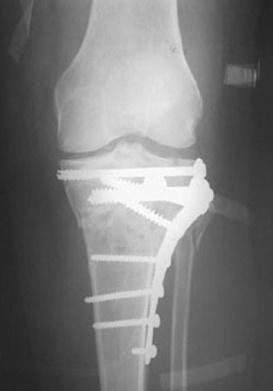
\includegraphics[width=0.25\textwidth]{001/image3.jpeg}
\end{figure}

\subparagraph{Fissazione esterna}
Si applicano viti o chiodi stabilizzati tra loro mediante un fissatore esterno che permette anche la riduzione della frattura. Viene preferita quando si ha un grosso rischio di infezione o in caso di fratture in determinate sedi: bacino, tibia e avambraccio (Nell'immagine: fissatore esterno).

\begin{figure}[!ht]
\centering
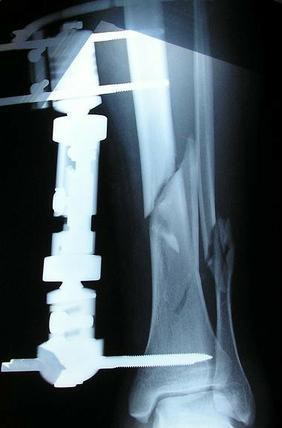
\includegraphics[width=0.25\textwidth]{001/image4.jpeg}
\end{figure}

\subparagraph{Sintesi endomidollari}
E' la più attuale! Sfrutta infibuli intra midollari che stabilizzano le fratture dall'interno. Questa metodica sfrutta la riparazione biologica col callo osseo periosteo diversamente dalla riparazione interna in cui si attua un'interruzione del processo ripartivo (Nell'immagine: chiodo Gamma).
  
\begin{figure}[!ht]
\centering
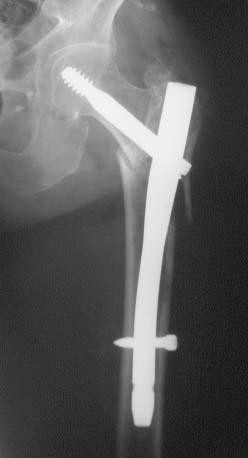
\includegraphics[width=0.25\textwidth]{001/image2.jpeg}
\end{figure}


In determinati casi le fratture non sono riparabili o meglio non conviene ripararle. Questo succede soprattutto negli anziani perché l'allettamento e la riabilitazione determinerebbero un crollo psicofisico ben peggiore della frattura stessa (sindrome da allettamento).

A questo punto il professore mostra un video di un intervento chirurgico di riduzione di una frattura e stabilizzazione chirurgica della stessa.
(Alcuni concetti precedenti vengono ripresi) Si tratta di una frattura del terzo distale della tibia. Viene mostrata la radiografia che conferma il sospetto diagnostico: si tratta di una frattura spiroide
scomposta (tipica frattura da torsione) in cui i due segmenti ossei non sono a contatto tra di loro. La frattura è stata trattata in sala operatoria sotto controllo endoscopico e per l'immobilizzazione la
scelta è stata quella della sintesi con chiodo endomidollare.

\begin{figure}[!ht]
\centering
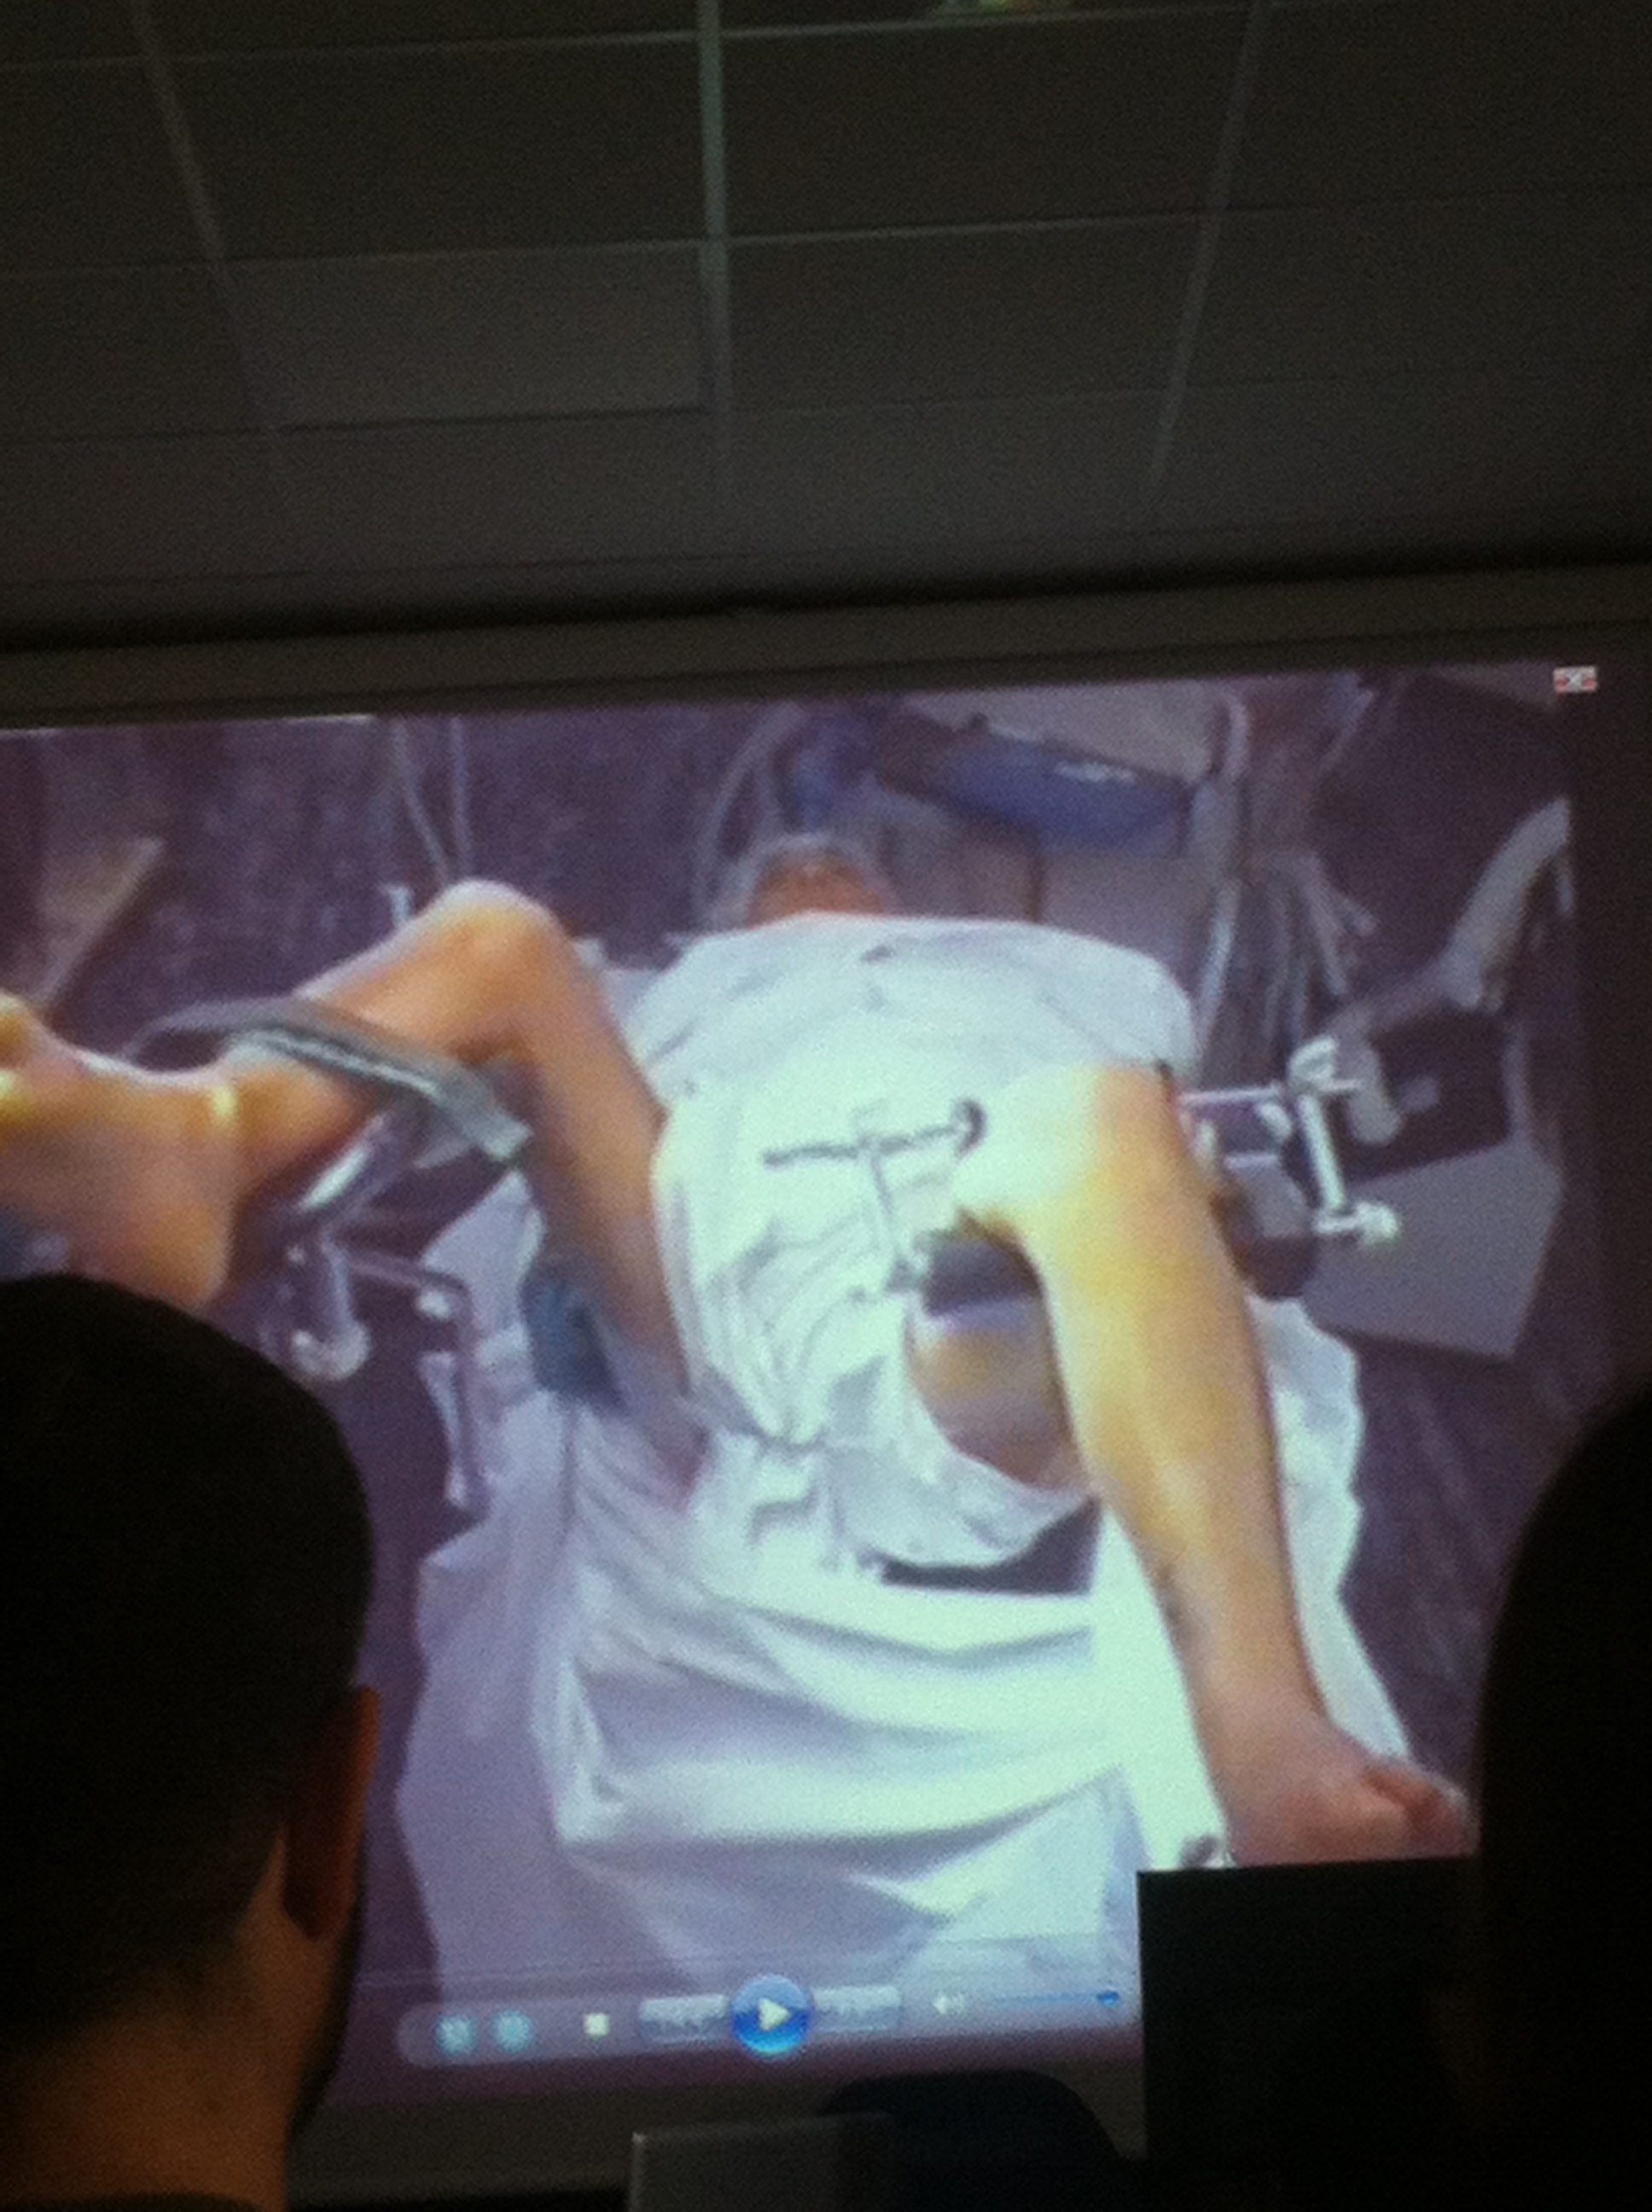
\includegraphics[width=0.3\textwidth]{001/image8.jpeg}
\end{figure}

La manovra di riduzione molto spesso viene eseguita sotto controllo dei raggi e si ricorre a posizioni particolari che facilitano la manovra stessa di riduzione e il posizionamento del chiodo (in questo caso il paziente è disteso sul lettino con le gambe sollevate). Molto spesso di fronte a una frattura delle ossa lunghe il paziente viene messo in \emph{trazione trans-scheletrica}: metodologia attuata per ridurre la
frattura e generalmente applicata in pronto soccorso in anestesia locale. Lo scopo di tale manovra è quello di \emph{trazionare progressivamente la frattura in vari segmenti corporei}: vengono progressivamente sgranati i frammenti della frattura e tesi i tessuti molli al fine di ridurre il gonfiore. Si tratta a tutti gli effetti di una parziale riduzione che verrà completata in seguito chirurgicamente. Ha il vantaggio di agevolare la fase chirurgica stessa. In questo caso è
stato posizionato il filo di trazione al calcagno e al letto vengono applicati pesi in kg che garantiscano la trazione.

Tali pesi devono essere pari al 5-10\% del peso corporeo per cui ad esempio per una frattura scomposta di femore in un soggetto di 70-80 kg si utilizzeranno pesi di 3,5/7 Kg. Importante ricordare i rischi legati
alla procedura stessa: un'eccessiva trazione può determinare eccessivo stiramento e parestesie o formicolio degli arti che devono essere necessariamente risolte.

A questo punto viene spiegata la procedura eseguita.. Attraverso proiezioni antero-posteriori e laterali il chirurgo controlla la fase di inserimento e procede alla riduzione della frattura. Questa manovra può
essere realizzata con l'ausilio di pinze o attraverso la cute previa incisione per raggiungere il focolaio della frattura. Nel video mostrato il chirurgo procede con incisione cutanea tramite la quale accede al
focolaio di frattura. A seguito della riduzione si procede con la \emph{stabilizzazione} che nel caso mostrato viene realizzata attraverso l'inserimento di un chiodo endomidollare che viene bloccato sopra e
sotto la frattura per dare stabilità. I chiodi sono cannulati, con buchi all'interno e necessitano dell'inserimento di un filo guida nel canale
midollare. Prima dell'inserimento del chiodo, si fresa il canale
midollare di uno o due mm in più del diametro del chiodo scelto, manovra
chiamata \textbf{ALESAGGIO DEL CANALE MIDOLLARE}.
\\\\
NB: Il chiodo a battuta viene posizionato solo se in tutte le proiezioni la frattura è riportata in posizione corretta! La punta del chiodo supera il focolaio di frattura e una volta posizionato con precisione verrà bloccato prossimalmente e distalmente con delle viti. Nel chiodo ci sono fori per le viti che posizionate perpendicolarmente vanno a bloccare il
chiodo sotto la frattura e in alto, sopra la stessa.

\begin{figure}[!ht]
\centering
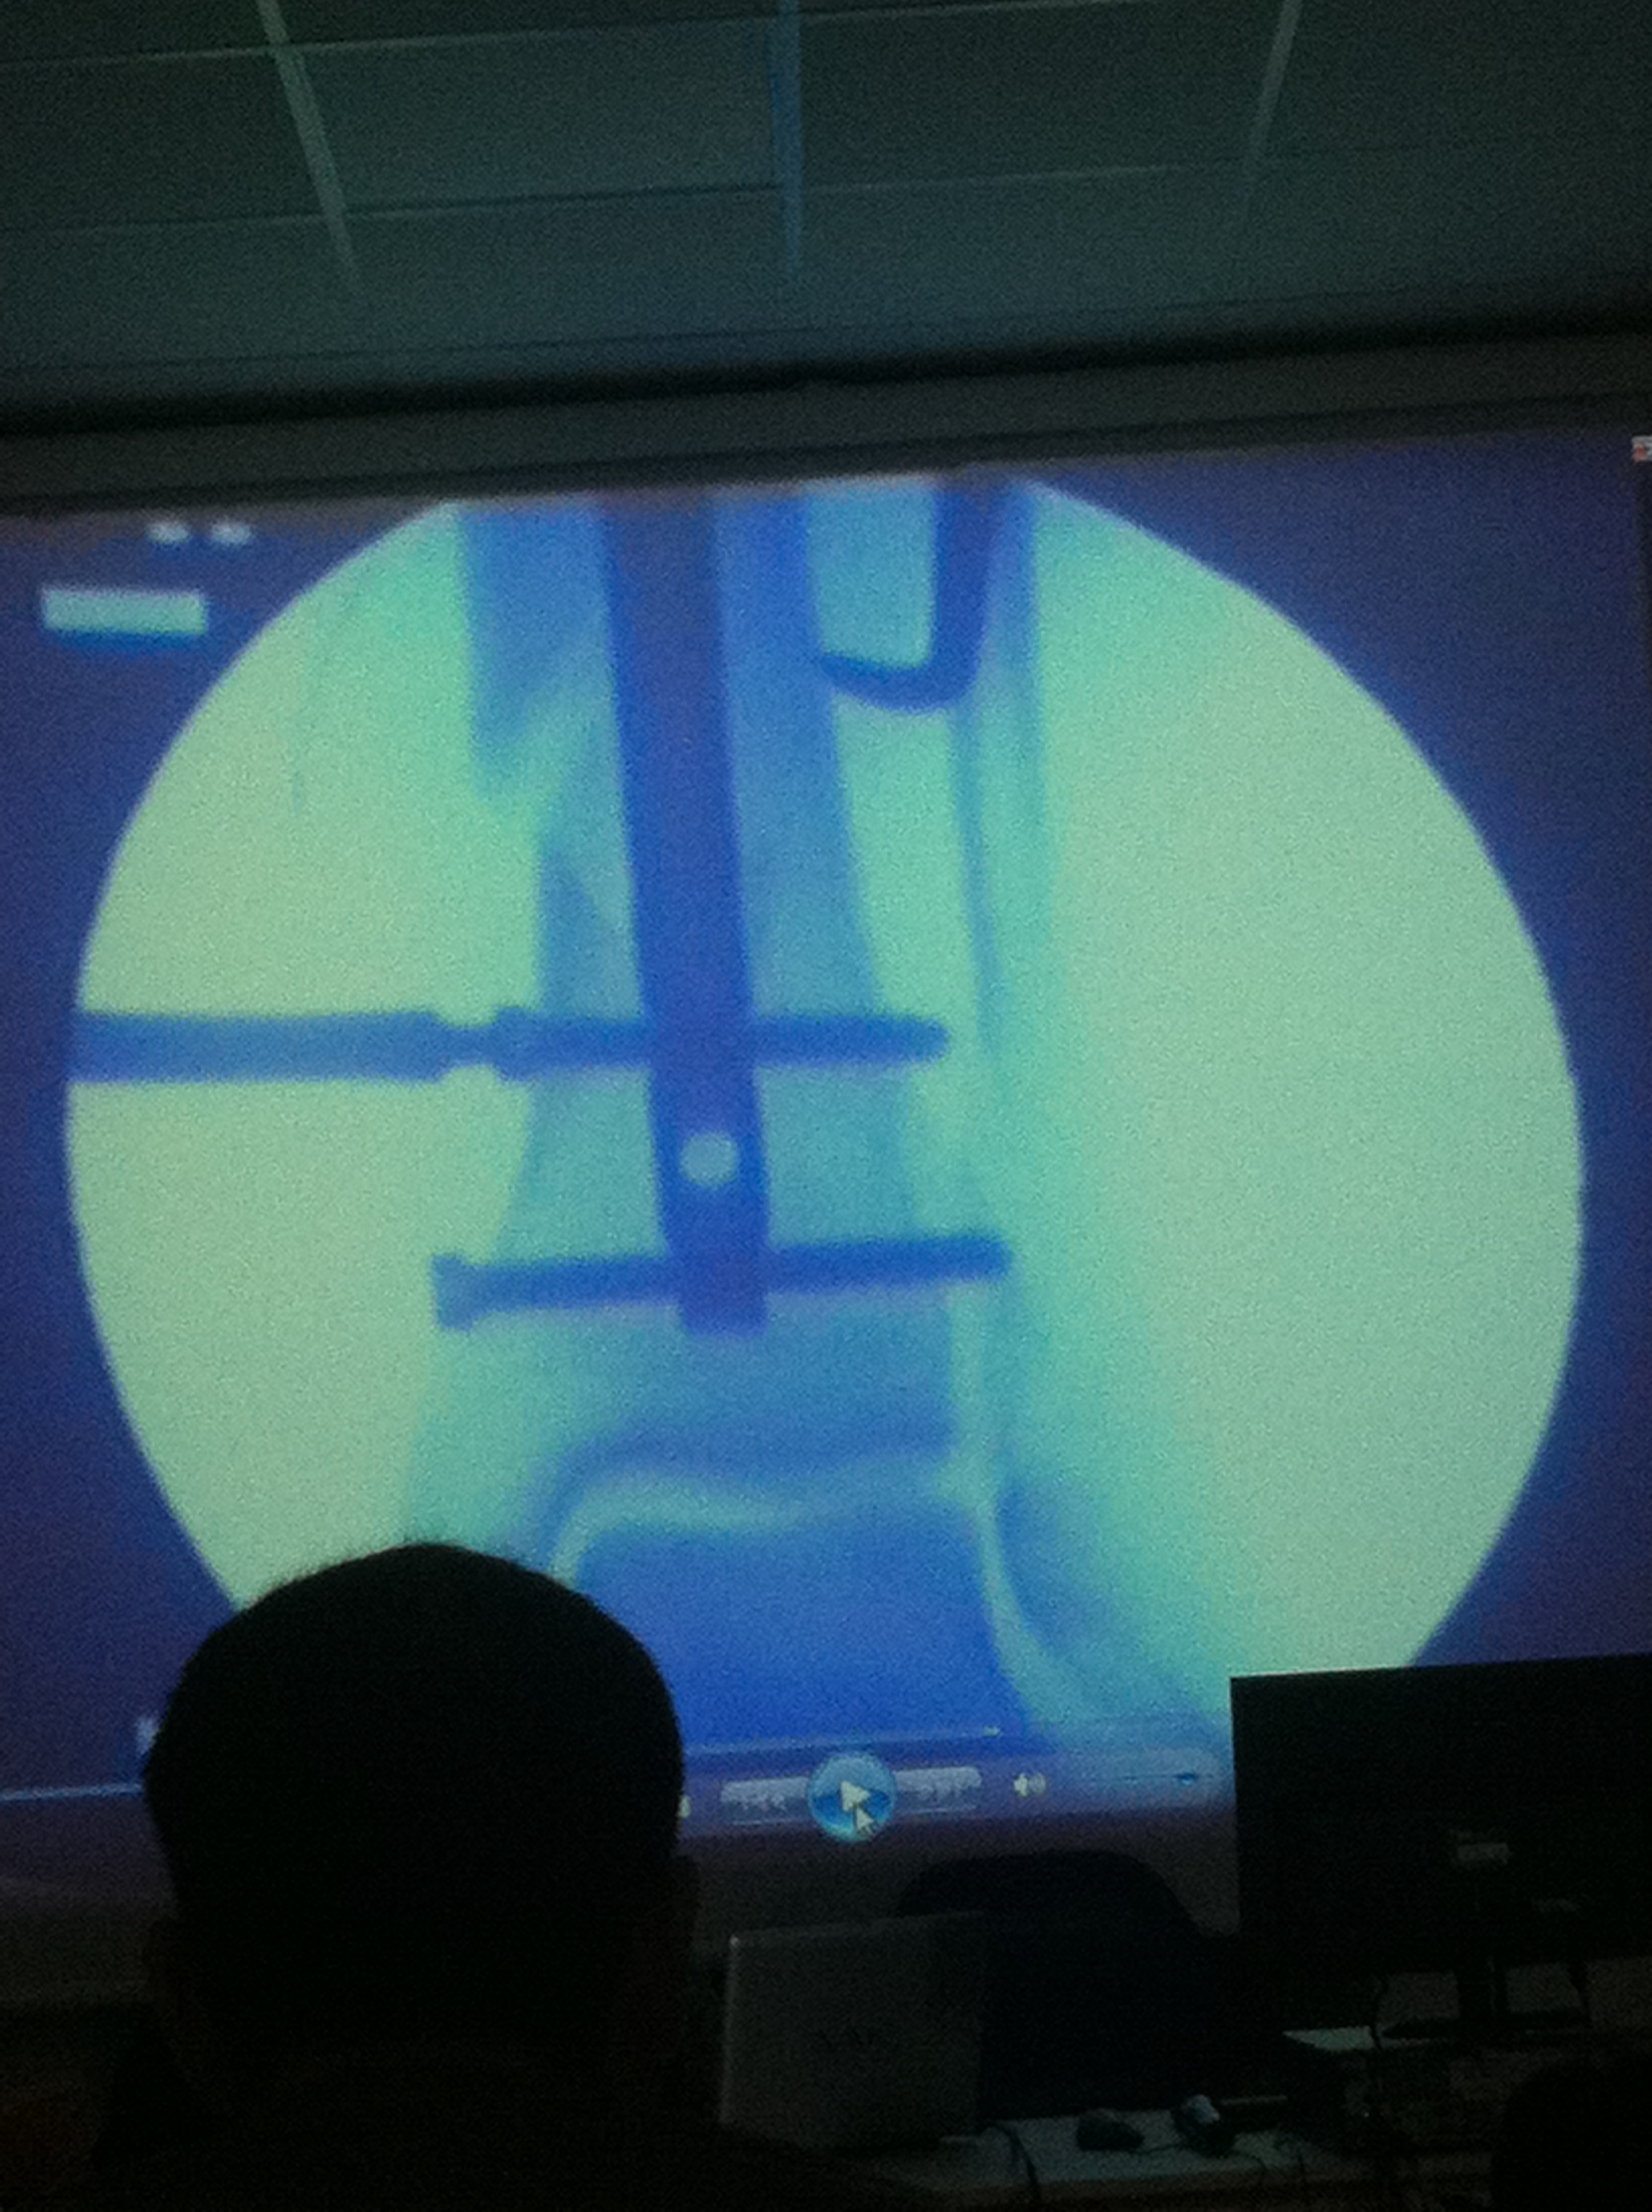
\includegraphics[width=0.3\textwidth]{001/image9.jpeg}
\end{figure}

PER RIASSUMERE:
\begin{itemize}
\item Diagnosi radiografica
\item Riduzione della frattura manuale o chirurgica (a cielo aperto con incisione o percutaneo con pinze)
\item Stabilizzazione della frattura: attraverso tutori, gesso, mezzi di sintesi inseriti chirurgicamente per favorire la guarigione.
\end{itemize}

La maggior parte delle fratture viene oggi trattata chirurgicamente, soprattutto se interessano le ossa lunghe. La chirurgia permette una riduzione migliore e una riabilitazione più rapida per cui minor incidenza di complicanze legate all'allettamento delle persone anziane e di complicanze locali come rigidità articolari. Il lavoro dell'ortopedico deve sempre andare di pari passo al lavoro del fisiatra/fisioterapista per ottenere il pieno recupero funzionale.

\newpage

\paragraph{\emph{Informazioni sul corso, tirocinio, modalità di svolgimento dell'esame:}}

\emph{Ortopedia e traumatologia: 3 cfu }

\emph{Medicina fisica e riabilitazione: 2 cfu }

\emph{TIROCINIO: Il tirocinio ha una durata di una settimana (Lun- Ven).
Sul sito è presente l'elenco delle settimane disponibili. Non più
disponibile reumatologia. Si viene suddivisi al mattino nelle varie
postazioni: ambulatorio traumi, pronto soccorso, medicina fisica e
riabilitazione.}

\emph{A tirocinio ogni giorno c'è un modulo in cui far apporre timbro e
firma del tutor, a fine settimana bisogna lasciare il libretto in
Segreteria (secondo piano Ortopedia, signora Giovanna). Ricordarsi di
presentare il libretto firmato all'esame!!}

\emph{In sala operatoria si può eccedere solo se interessati, è
necessario fare richiesta. C'è la possibilità di fare tirocinio a
Fidenza o Piacenza, comunicarlo per tempo al prof Coordinatore del corso
(prof. Pogliacomi).}

\emph{Se interessati alla materia si può frequentare il reparto.
Possibilmente iscriversi il prima possibile ai tirocini, in vicinanza
dell'esame. \emph{NB: Da sostenere entro l'anno accademico!} Le date dei
tirocini sono tutte sul sito, iscrizione online.}

\emph{ESAME: orale, iscrizione online e registrazione online. L'esame si
compone di 3 domande, riguardanti le materie del corso (una di
ortopedia, una di traumatologia, una di medicina fisica e
riabilitazione). Un prof può chiedere tutte e tre le domande o solo una:
è variabile! Il voto finale è costituito dalla media dei tre voti.
\emph{Tutte e tre le domande devono essere sufficienti per passare
l'esame}.}

\emph{I testi consigliati si trovano sul sito del corso.}
